\documentclass[a4paper]{article}
\usepackage{graphicx}
\usepackage{twocolceurws}
\usepackage{amsmath}
\usepackage{xcolor}


\title{Specified Backup for Fragile Parts of LLMs}

\author{
Abhi Morumpalle
\and
Allen Zhang
\and
Arnav Marda
\and
Jeffrey Kwan
\and
Harry Qian
}

\institution{Team A5}




\begin{document}
\maketitle

\begin{abstract}
In the past few years, there has been an explosion of interest in Large Language Models (LLMs) for a variety of practical applications. Much of this explosion has been driven by the invention of the Transformer architecture \cite{Vaswani17}. However, the Transformer architecture inner workings largely remain a mystery. Combining this with the applications that LLMs are finding in the real-world, there a variety of new security risks that these LLMs open
up their users to. In this paper, we analyze the robustness of LLMs to random bitflips in the variables, pinpointing specific parts of the LLM that are vulnerable to these hardware errors.


\end{abstract}


\section{Introduction}

In the past few years, there has been an explosion of interest in LLMs with the creation of widely available resources like OpenAI's ChatGPT
and Meta's open source Llama. Much of the explosion has been driven by the creation of the transformer architecture, which has made a dramatic difference throughout AI, but particularly in the world of LLMs. However, our fundamental understanding of how these objects remains shrouded in mystery.

Because of our lack of understanding of how these objects work, and the quick assimilation of these products into our daily lives, there are a variety of novel security risks that we are being introduced to. One specific error is not so common, but still of practical relevance, is a hardware failure in which a random bitflip occurs in the parameters of our model. An error of such a fashion could have drastic effects on our output, ranging from making the outputs gibberish to outright wrong.

In this paper, we analyze how injecting bit errors into specific locations of a transformer and the LLM model as a whole affect the output. To this end, we use the GPT2 as a base model to test on. To inject errors into our base model we use the PyTEI package \cite{Ma23}. To quantify the effect of our errors, we compare the score of our base model to the score of the models with errors injected using the PyTEI package with DeepEval to evaluate.


Our basic workflow is outlined in the below diagram

\begin{figure}[ht]
	\begin{center}
		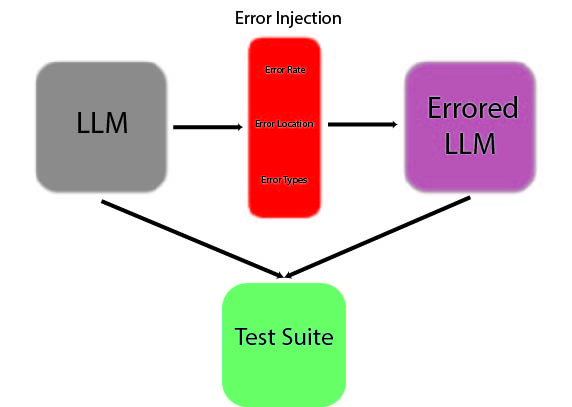
\includegraphics[height=6cm]{workflow.jpg}
		\caption{General evaluation workflow for LLM}
		\label{workflow}
	\end{center}
\end{figure}

\section{Threat Model}
We present 2 case studies, relating to information disclosure and denial of service respectively. \\

An attacker's goal is to cause information disclosure or cause a denial of service via system crash or significantly degrading the performance of the LLM. They may attack components such as edge AI chips and accelerators, CPUs and GPUs in LLM training, memory systems storing model weights, and data transfer channels between hardware components. To induce hardware errors, they could somehow achieve write access to memory systems, or physical access to create fault-heavy environments (e.g. radiation source). 

\subsection{Case Studies}
case 1 (information disclosure): An LLM is running on an edge device (like a smartwatch). The attacker jailbreaks the device, gaining write access to hardware, and inject bit errors with a probability $p$. The attacker then monitors the LLM output through API calls, observing that the output is NaN XX\% of the time. The attacker thus concludes that the LLM has YY number of parameters (see \textcolor{red}{how to cite analysis of nan section} for more details). \\

case 2 (denial of service): A physics research lab is using LLMs for running simulations of their experiments. An attacker somehow manages to convince the lab scientists to house the servers the LLM is running on in their reactor chamber, a source with high radiation. This environment causes many bit flip errors, causing frequent faulty outputs from the LLM.

For the purposes of this paper, we will investigate the effects of the denial of service attack objective, specifically performance degradation.


[todo: make a figure of the threat model]

\section{Project Goals and Timeline}

The goal of this project is to evaluate the effect of random bit flips on the output of LLMs and analyze the possible security hazards that these hardware errors could cause in real systems. We plan to do this by modeling various rates of bit flips and by injecting errors into various parts of the LLMs, and evaluating the robustness on a variety of different tests.

Up until now, we have chosen a open source model that gives us the freedom to inject various bit errors, and have select some tests that we can evaluate our models on. There are still multiple tests that we want to evaluate our model on, and some more analysis to be done to find specific places to inject bit flips into to look for any particularly vulnerable parts.

Below is a general timeline for what we want to accomplish and when.

\begin{itemize}
	\item Week 7: Finish selecting different tests to evaluate
	\item Week 8: Try injecting vulnerabilities into specific parts of the LLM with different error rates
	\item Week 9: Analyze results and compile into final report
	\item  Week 10: Finish final report and presentation
\end{itemize}

Using this, we can turn the knobs to evaluate different kinds of error and add various tests to our test-suite as we continue to expand our results.


\section{Methods}

We chose Hugging Face's implementations of GPT-2 \cite{gpt2} as our model of choice. We evaluated our models on \cite{DeepEval}, an open-source LLM benchmark, specifically the computer science and astronomy tests that have the injected LLM answer multiple choice questions. For each model with varying error rates, the score is computed as the proportions of correct answers. For the purposes of this midterm report, we only implemented coarsed-grained error injection into every layer.


\section{Preliminary Results}
\begin{figure}[ht]
	\begin{center}
		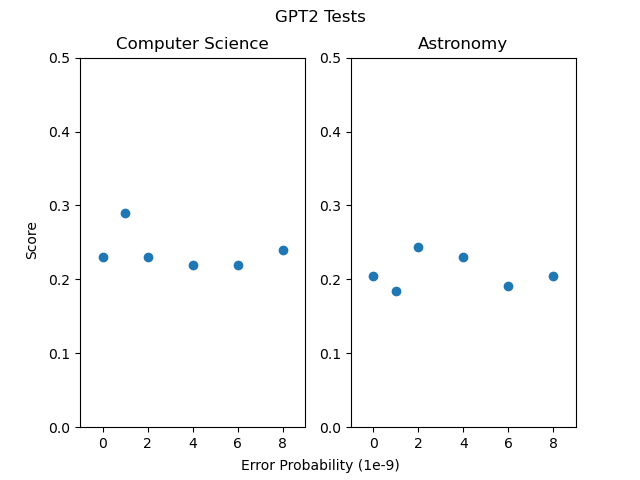
\includegraphics[height=6cm]{gpt2.png}
		\caption{GPT 2 performance on DeepEval with varying error rates}
		\label{gpt2-res}
	\end{center}
\end{figure}

As seen in Figure \ref{gpt2-res}, we see a negligable change in performance varying error rates in the range of 1e-9 on both benchmarks. Note that we were unable to increase the error rate anything beyond that because it resulted in a NaN output. This is likely due to the fact that random bit flips happened in the exponent field of a number.

However, the results tended to be have large deviation from one run to the other and because of our limited computation resources were were not able to finish enough runs in the required time to get a solid average. In addition, the number of errors that are injected are a probablistic sample, which also makes the results less certain for these fewer number of runs. This is a strong limitation of our work so far.

However, our current work does indicate that perhaps LLMs remain quite robust to a small number of errors, which would be the relevant case for random hardware bitflips induced by strictly hardware errors.

\section{Analysis of NaN}
In this section, we provide an analysis of the probability that the LLM outputs NaN. \\

Let $F$ be an LLM model with $n$ parameters and $x$ be the input to the model. We would like to find $Pr(F(x) = NaN)$.

Suppose a bit is flipped with probability $p$.

Let $X$ be the value of a model parameter and $X^*$ be its perturbed value. Note that parameters are iid $\sim Uniform(0, 1)$ due to the design of LLMs [do you have a good source for this allen]. According to \cite{IEEE754}, a NaN value has all 1s in the exponent field, and a nonzero mantissa. Since $0 \le X \le 1$, the exponent field is $01111111$ (due to the +127 offset), and suppose there are $j$ 1s in the mantissa. \\

Then, $X^* = NaN$ if the remaining exponent bit flipped, the rest of the exponent bits don't flip, and not all $j$ mantissa bits turn to 0. Thus,

\begin{align*}
	Pr(X^* = NaN) &= Pr(\text{only one exponent bit is flipped}) \cdot (1 - Pr(\text{all mantissa bits are 0})) \\
	&= p(1 - p)^7 * (1 - p^j(1 - p)^{23 - j})
\end{align*}

We can represent the value of mantissa as a random variable $\sim Binom(23, 0.5)$. Thus,

\begin{align*}
	Pr(X^* = NaN) &= \sum_j^23 Pr(X^* = NaN \mid X \text{ has $j$ mantissa 1s})Pr(X\text{ has $j$ mantissa 1s}) \\
	&= \sum_j^23 p(1 - p)^7 * (1 - p^j(1 - p)^{23 - j})\binom{23}{j}0.5^j0.5^{23 - j} \\
	&= 2^{-23} p (1 - p)^7 \left(\sum_{j=0}^{23}[1 - p^j(1 - p)^{23 - j}] \binom{23}{j}\right) \\
	&= 2^{-23} p (1 - p)^7 \left(\sum_{j=0}^{23}\binom{23}{j} - \sum_{j=0}^{23}p^j(1 - p)^{23 - j} \binom{23}{j}\right) \\
	&= 2^{-23} p (1 - p)^7(2^23 - 1)
	&= p(1 - p)^7(1 - 2^{-23})
\end{align*}

Now putting everything together, we note that the model will output NaN if any of the parameters of the model are NaN, due to NaN propagation. Thus,

\begin{align*}
	Pr(F(x) = NaN) &= Pr(\text{at least one parameter is NaN}) \\
	&= 1 - Pr(\text{all parameters are not NaN}) \\
	&= 1 - \prod_{i=1}^n Pr(X_i \neq NaN) \\
	&= 1 - Pr(X^* \neq NaN)^n \\
	&= 1 - (1 - Pr(X^* = NaN))^n \\
	&= 1 - (1 - p(1 - p)^7(1 - 2^{-23}))^n
\end{align*}

For $p = 10^{-9}$ and $n \approx 130 * 10^6$ (GPT-2), we get $Pr(F(x) = NaN) \approx 0.1$, and for $p = 10^{-8}$, we get $Pr(F(x) = NaN) \approx 0.7$, which explains why at a low error rate, the model still outputs NaN quite consistently.

\section{Future Work}

From a results standpoint, we hope to be able to find the time to run more tests to get a stronger average. We also hope to be able to modify PyTEI to inject a random number of errors, instead of using a low probability of injecting errors which has a large variance of the number of errors that are actually injected. In addition, some errors tend to be much more severe than others, which again raises the variance in our testing. This compounded with the fact that the appearance of NaN values stops us from evaluating high bit Thus, we hope to be able to modify PyTEI to support our more specific cases.

From a better testing standpoint, in the near future, we hope to be able to pick more tests that can evaluate the effect of bit flips on our model. This will take a significant amount of compute time, even though we have chosen a mini LLM model.

For future work, we hope to be able to analyze our different parts of the LLM are affected by random bit flips. For example, we want to see if a bit flip in the attention mechanism is more relevant than a bit flip in the fully connected layeres, or vice versa. 

In addition, because of the bits being stored as a floating point, it's also possible that some bit flips can be much more relevant than others. For example, a bit being flipped in the exponent produces a much larger effect than a bit being flipped in the mantissa. We hope to be able to expand on the PyTEI library to give us the ability to evaluate these effects.

Furthermore, it may be worth taking some time to evaluate larger, more modern models to see if more accurate models tend to be less robust.

Using this larger body of results, we hope to be able to analyze the possible security risks that hardware errors pose to LLM implementations.

\section{Related Work}
There is a related paper \cite{Ma23} that analyzes a model known as a recommendation system. In their work, they build the PyTEI package for injecting models. However, recommendation models differ significantly from LLMs so the overall effect could be quite different for the same error injections.

However, the paper does not do any evaluation on the different of hardware errors in specific parts of the recommendation system, so the question of whether particular parts are more vulnerable is still open.

An interesting part of this paper is the evaluation of possible mitigations against hardware flips, which can also be evaluated in the context of LLMs. In addition, their evaluation had limited scope, and it could be interesting to expand on their analysis by testing a wider variety of errors and examining the tradeoffs of each.

\cite{fidelity} performed resilience analysis on transient errors in logic components, but their framework is highly inefficient in the context of PyTorch, because they employ frequent to-and-back type conversions as PyTorch doesn't natively support bit operations in float tensors. \cite{thales} estimated DNN accuracy under transient faults and proposed a Monte Carlo-based estimation method. However, their analysis is also limited to transient errors and do not consider logic / data path errors which are permanent and more impactful.

\begin{thebibliography}{Com79}

\bibitem[He et. al, 2020]{fidelity} Yi He, Prasanna Balaprakash, and Yanjing Li. 2020. Fidelity: efficient resilience analysis framework for deep learning accelerators. In 2020 53rd Annual IEEE/ACM International Symposium on Microarchitecture (MICRO). IEEE, 270–281.

\bibitem[Abhishek et. al, 2022]{thales} Abhishek Tyagi, Yiming Gan, Shaoshan Liu, Bo Yu, Paul Whatmough, and Yuhao Zhu. 2022. Thales: formulating and estimating architectural vulnerability factors for dnn accelerators. arXiv preprint arXiv:2212.02649

\bibitem[Vaswani et. al, 2017]{transformer} Vaswani, Ashish, et al. 
\newblock"Attention is all you need."

\bibitem[Ma et al., 2023]{Ma23} D. Ma, X. Jiao, F. Lin, M. Zhang, A. Desmaison, T. Sellinger, D. Moore, S. Sankar.
\newblock Evaluating and Enhancing Robustness of Deep Recommendation Systems Against Hardware Errors

\bibitem[DeepEval]{DeepEval} Confident AI.
\newblock DeepEval: The LLM Evaluation Framework. Retrieved from https://github.com/confident-ai/deepeval.

\bibitem[Radford et al., 2019]{gpt2} Radford, Alec and Wu, Jeff and Child, Rewon and Luan, David and Amodei, Dario and Sutskever, Ilya. 
\newblock Language Models are Unsupervised Multitask Learners

\bibitem[IEEE-754, 2019]{IEEE754} IEEE. 
\newblock 754-2019 - IEEE Standard for Floating-Point Arithmetic.

\end{thebibliography}
\end{document}
